\section{Results}
\label{sec:action_results}




\subsection{3d geometric reasoning algorithm}

Three cluttered kitchen scenarios are used for benchmarking the algorithm; they are shown in \figref{fig:sec_enriched_geometricalreasoning_experiments_scenesexample}.
They are recorded using an Asus Xtion Pro camera, which records RGB as well as depth information.
First, in \figref{fig:sec_enriched_geometricalreasoning_experiments_scenesexample_scenes1} a cup is next to a box and an apple is on top of a pedestal.
In the second scenario, \figref{fig:sec_enriched_geometricalreasoning_experiments_scenesexample_scenes2}, two plates are lying around: on on top of a cutting board, the other one on a table.
This plate is filled with an apple and a pedestal, and on top of the pedestal there is an empty jar.
Lastly, in \figref{fig:sec_enriched_geometricalreasoning_experiments_scenesexample_scenes3}, a cluttered scene containing a green apple touching a blue cup, two spoons on a spoon holder, an orange on top of a board, a knife in a knife holder, and a red pedestal in the background is introduced.
While arguably all three scenarios are not very likely to be found in a kitchen outside a lab environment, they serve as a good example for cluttered objects, which are randomly stacked or lying around in close vicinity to each other.

\begin{figure}
  \begin{subfigure}[]{0.32\textwidth}
    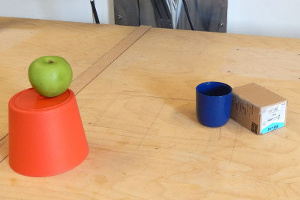
\includegraphics[width=\textwidth]{./figures/sec/scene_photos/affordance_scene4_wide.jpg}
    \caption{Scene 1.}
    \label{fig:sec_enriched_geometricalreasoning_experiments_scenesexample_scenes1}
  \end{subfigure}
  \hfill
  \begin{subfigure}[]{0.32\textwidth}
    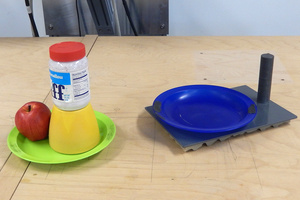
\includegraphics[width=\textwidth]{./figures/sec/scene_photos/affordance_scene7_wide.jpg}
    \caption{Scene 2.}
    \label{fig:sec_enriched_geometricalreasoning_experiments_scenesexample_scenes2}
  \end{subfigure}
  \hfill
  \begin{subfigure}[]{0.32\textwidth}
    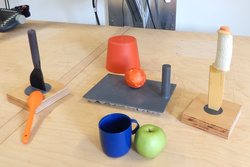
\includegraphics[width=\textwidth]{./figures/sec/scene_photos/affordance_scene5_wide1.jpg}
    \caption{Scene 3.}
    \label{fig:sec_enriched_geometricalreasoning_experiments_scenesexample_scenes3}
  \end{subfigure}
  \caption{Three different scenes are used to test the algorithm. They resemble cluttered kitchen scenarios as one might expect them in the real world.}
  \label{fig:sec_enriched_geometricalreasoning_experiments_scenesexample}
\end{figure}

Qualitative results of geometric reasoning are shown for the first scene in \figref{fig:sec_enriched_geometricalreasoning_experiments_scene1}, for scene 2 in \figref{fig:sec_enriched_geometricalreasoning_experiments_scene2}, and for scene 3 in \figref{fig:sec_enriched_geometricalreasoning_experiments_scene3}.
These results show that by processing the low level point clouds one can detect the blocked and free directions of a given object.
Thereafter, quantitative results are presented.

\begin{figure}
  \centering
  \begin{subfigure}[t]{0.475\textwidth}
    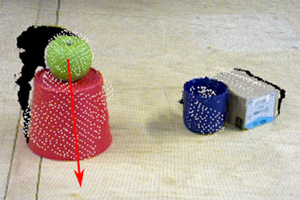
\includegraphics[width=1.0\textwidth]{./figures/sec/geometrical_reasoning/affordance_arrow_scene4_1.jpg}
    \caption{Apple and red pedestal. The arrow points to the front and bottom.}
    \label{fig:sec_enriched_geometricalreasoning_experiments_scene1_1}
  \end{subfigure}
  \hfill
  \begin{subfigure}[t]{0.475\textwidth}
    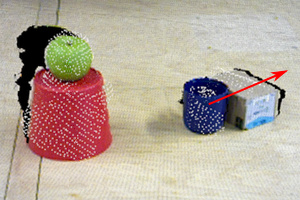
\includegraphics[width=1.0\textwidth]{./figures/sec/geometrical_reasoning/affordance_arrow_scene4_2.png}
    \caption{Cup and box. The arrow points towards the box.}
    \label{fig:sec_enriched_geometricalreasoning_experiments_scene1_2}
  \end{subfigure}
  \caption{Qualitative results for the geometrical reasoning method, scene 1. Recorded depth points on the objects are marked using white dots. The algorithm is applied to the object pair apple and red pedestal, and blue cup and box. For graphical purposes only the lar\-gest cluster is shown with a red arrow. Here, the arrow points from the apple downwards to the pedestal, which is the ``forbidden'' direction, if you want to lift the apple.}
  \label{fig:sec_enriched_geometricalreasoning_experiments_scene1}
\end{figure}

\begin{figure}
  \centering
  \begin{subfigure}[t]{0.475\textwidth}
    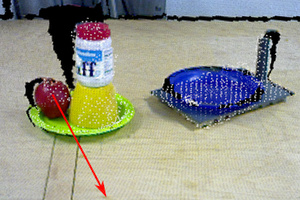
\includegraphics[width=\textwidth]{./figures/sec/geometrical_reasoning/affordance_arrow_scene7_1.jpg}
    \caption{Apple and green plate. The arrow is pointing to the front and not to the plate.}
    \label{fig:sec_enriched_geometricalreasoning_experiments_scene2_1}
  \end{subfigure}
  \hfill
  \begin{subfigure}[t]{0.475\textwidth}
    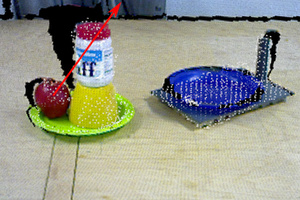
\includegraphics[width=\textwidth]{./figures/sec/geometrical_reasoning/affordance_arrow_scene7_2.jpg}
    \caption{Apple and jar. The arrow is pointing towards the jar.}
    \label{fig:sec_enriched_geometricalreasoning_experiments_scene2_2}
  \end{subfigure}\\%
  \begin{subfigure}[t]{0.475\textwidth}
    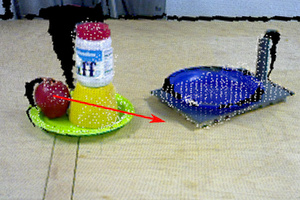
\includegraphics[width=\textwidth]{./figures/sec/geometrical_reasoning/affordance_arrow_scene7_3.jpg}
    \caption{Apple and yellow pedestal. The arrow is pointing towards the yellow pedestal.}
    \label{fig:sec_enriched_geometricalreasoning_experiments_scene2_3}
  \end{subfigure}
  \hfill
  \begin{subfigure}[t]{0.475\textwidth}
    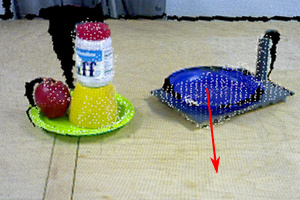
\includegraphics[width=\textwidth]{./figures/sec/geometrical_reasoning/affordance_arrow_scene7_4.png}
    \caption{Plate and board. Here, too, the arrow points as expected.}
    \label{fig:sec_enriched_geometricalreasoning_experiments_scene2_4}
  \end{subfigure}
  \caption{Qualitative results for the geometrical reasoning method for scene 2. For graphical purposes only the largest cluster is shown with a red arrow.}
  \label{fig:sec_enriched_geometricalreasoning_experiments_scene2}
\end{figure}

\begin{figure}[]
  \centering
  \begin{subfigure}[t]{0.475\textwidth}
    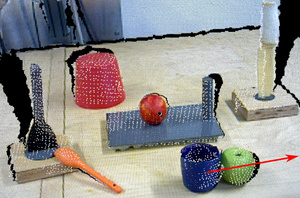
\includegraphics[width=\textwidth]{./figures/sec/geometrical_reasoning/affordance_arrow_scene5_1.jpg}
    \caption{Scene 3: Blue cup and apple. The arrow points towards the apple}
    \label{fig:sec_enriched_geometricalreasoning_experiments_scene3_1}
  \end{subfigure}
  \hfill
  \begin{subfigure}[t]{0.475\textwidth}
    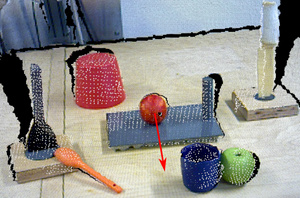
\includegraphics[width=\textwidth]{./figures/sec/geometrical_reasoning/affordance_arrow_scene5_2.jpg}
    \caption{Scene 3: Orange and board. The arrow points slightly to the front and bottom.}
    \label{fig:sec_enriched_geometricalreasoning_experiments_scene3_2}
  \end{subfigure}\\%
  \begin{subfigure}[t]{0.475\textwidth}
    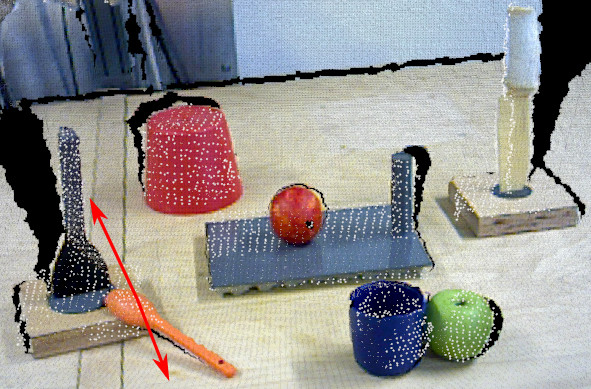
\includegraphics[width=\textwidth]{./figures/sec/geometrical_reasoning/affordance_arrow_scene5_3.jpg}
    \caption{Scene 3: Orange spoon and black spoon. The largest cluster points towards the black spoon, the second largest cluster points downwards.}
    \label{fig:sec_enriched_geometricalreasoning_experiments_scene3_3}
  \end{subfigure}
  \caption{Qualitative results for the geometrical reasoning method for a cluttered scene. For graphical purposes only the largest cluster is shown with a red arrow. Please note the two red arrows in (c). Here, the two largest clusters are depicted.}
  \label{fig:sec_enriched_geometricalreasoning_experiments_scene3}
\end{figure}

However, the quality of the direction computed also depends on the quality of the recorded point cloud data.
For perfect results, points on every side of the object are needed.
In real-world scenarios usually only one side is recorded, which means, that the computed normals are sometimes off.
For example, in \figref{fig:sec_enriched_geometricalreasoning_experiments_scene2_1}, which shows the spatial relation between an apple and a green plate, the arrow points downwards, but also to the side.
There are no points on the apple recorded, which could point downwards.
The resulting arrow points to the front.
However, the directions to the two objects in front of the apple, the jar (\figref{fig:sec_enriched_geometricalreasoning_experiments_scene2_2}) and yellow pedestal (\figref{fig:sec_enriched_geometricalreasoning_experiments_scene2_3}) are found correctly.

Another problem can be seen in \figref{fig:sec_enriched_geometricalreasoning_experiments_scene3_3} showing scene 3.
Here, the relations between the orange spoon and the black spoon in the spoon holder (black spoon and spoon holder are recognized as one object) form one unexpected cluster downwards, all others point towards the spoon.
Careful examinations show that there actually are some points belonging to the spoon base below the orange spoon and that the arrow downward is justified.
However, the resulting access angle is very small.

For a quantitative analysis, ground truth needs to be generated first.
For the following analysis, this was done manually.
For each object pair in each scene the access angles are defined.
Success is reported, if and only if the 3d-cone of the found angles is entirely within the cone defined by ground truth.
A negative result is issued when the cones overlap.
Instead of a binary outcome, one could define a percentage of overlap as quality measure.
However, false-positive errors are still dangerous in the robot execution part.
Each scene is recorded ten times via an Asus Xtion Pro sensor from different angles, but always front facing --- meaning the recordings are similar to the figures shown above (\figref{fig:sec_enriched_geometricalreasoning_experiments_scene1} -- \figref{fig:sec_enriched_geometricalreasoning_experiments_scene3}).
Results are shown in \tabref{tab:sec_resultsgeometricalreasoning_experiments_scene1}, \tabref{tab:sec_resultsgeometricalreasoning_experiments_scene2}, and \tabref{tab:sec_resultsgeometricalreasoning_experiments_scene3} for scene 1, 2, and 3 respectively.

\begin{table}[]
  \centering
  \begin{tabular}{l|cccc}
    \toprule
                & Apple   & Pedestal  & Blue cup  & Box\\
    \midrule
    Apple to    &         & 100\%     & 100\%     & 100\%\\
    Pedestal to & 70\%    &           & 70\%      & 70\%\\
    Blue cup to & 80\%    & 80\%      &           & 30\%\\
    Box to      & 10\%    & 10\%      & 10\%      &\\
    \bottomrule
  \end{tabular}
  \caption{Results for scene 1, see \figref{fig:sec_enriched_geometricalreasoning_experiments_scenesexample_scenes1}.}
  \label{tab:sec_resultsgeometricalreasoning_experiments_scene1}
\end{table}

\begin{table}[]
  \centering
  \begin{tabular}{l|cccccc}
    \toprule
                      & \rotatebox[origin=l]{90}{Red apple} 
                      & \rotatebox[origin=l]{90}{Pedestal} 
                      & \rotatebox[origin=l]{90}{Jar}       
                      & \rotatebox[origin=l]{90}{Green plate}
                      & \rotatebox[origin=l]{90}{Blue plate}
                      & \rotatebox[origin=l]{90}{Cutting board}\\
                      %& \multirow{2}{*}{Apple}& \multirow{2}{*}{Pedestal} & \multirow{2}{*}{Jar}      & Green       & Blue        & Cutting\\
                      %&                       &                           &                           & plate       & plate       & board\\
    \midrule
    Apple to          &                       & 100\%                     & 100\%                     & 0\%         & 100\%       & 100\%         \\
    Pedestal to       & 20\%                  &                           & 0\%                       & 10\%        & 30\%        & 30\%          \\
    Jar to            & 100\%                 & 0\%                       &                           & 0\%         & 100\%       & 100\%         \\
    Green plate to    & 0\%                   & 0\%                       & 100\%                     &             & 0\%         & 0\%           \\
    Blue plate to     & 100\%                 & 0\%                       & 100\%                     & 0\%         &             & 0\%           \\
    Cutting board to  & 100\%                 & 100\%                     & 100\%                     & 100\%       & 100\%       &               \\
    \bottomrule
  \end{tabular}
  \caption{Results for scene 2, see \figref{fig:sec_enriched_geometricalreasoning_experiments_scenesexample_scenes2}.}
  \label{tab:sec_resultsgeometricalreasoning_experiments_scene2}
\end{table}

\begin{table}[]
  \centering
  \begin{tabular}{l|ccccc}
    \toprule
                      & \rotatebox[origin=l]{90}{Red apple} 
                      & \rotatebox[origin=l]{90}{Green apple} 
                      & \rotatebox[origin=l]{90}{Blue cup}       
                      & \rotatebox[origin=l]{90}{Cutting board}       
                      & \rotatebox[origin=l]{90}{Pedestal}\\
                      % Apple     Green apple Blue cup    c board       pedestal
    \midrule
    Red apple to      &         & 100\%     & 100\%     & 0\%         & 0\%    \\
    Green apple to    & 0\%     &           & 20\%      & 0\%         & 0\%    \\
    Blue cup to       & 100\%   & 100\%     &           & 100\%       & 100\%  \\
    Cutting board to  & 100\%   & 100\%     & 100\%     &             & 30\%   \\
    Pedestal to       & 100\%   & 100\%     & 100\%     & 100\%       &        \\
    Knife to          & \xmark  & \xmark    & \xmark    & \xmark      & \xmark \\
    Knife holder to   & 100\%   & 100\%     & 100\%     & 100\%       & 100\%  \\
    Black spoon to    & 100\%   & 100\%     & 100\%     & 100\%       & 100\%  \\
    Orange spoon to   & 10\%    & 100\%     & 100\%     & 0\%         & 0\%    \\
    Spoon holder to   & 100\%   & 100\%     & 100\%     & 70\%        & 100\%  \\
    \bottomrule
  \end{tabular}
  \begin{tabular}{l|ccccc}
    \toprule
                      & \rotatebox[origin=l]{90}{Knife} 
                      & \rotatebox[origin=l]{90}{Knife holder} 
                      & \rotatebox[origin=l]{90}{Black spoon} 
                      & \rotatebox[origin=l]{90}{Orange spoon} 
                      & \rotatebox[origin=l]{90}{Spoon holder}\\
                       %knife                      k holder  b spoon o spoon  spoon holder
    \midrule
    Red apple to      & 0\%                     & 0\%     & 80\%  & 100\%   & 100\%\\
    Green apple to    & 0\%                     & 0\%     & 0\%   & 0\%     & 0\%\\
    Blue cup to       & 100\%                   & 100\%   & 90\%  & 90\%    & 90\%\\
    Cutting board to  & 100\%                   & 100\%   & 100\% & 100\%   & 100\%\\
    Pedestal to       & 100\%                   & 100\%   & 100\% & 100\%   & 100\%\\
    Knife to          &                         & \xmark  & \xmark& \xmark  & \xmark\\
    Knife holder to   & 100\%                   &         & 100\% & 100\%   & 100\%\\
    Black spoon to    & 100\%                   & 100\%   &       & 100\%   & 0\%\\
    Orange spoon to   & 60\%                    & 50\%    & 0\%   &         & 100\%\\
    Spoon holder to   & 100\%                   & 100\%   & 100\% & 100\%   &\\
    \bottomrule
  \end{tabular}
  \caption{Results for scene 3, see \figref{fig:sec_enriched_geometricalreasoning_experiments_scenesexample_scenes3}.}
  \label{tab:sec_resultsgeometricalreasoning_experiments_scene3}
\end{table}

They reflect the problems from the qualitative evaluation.
What one first notices, is the almost binary distribution of success and failure: The percentage computed is either very high or very low.
This leads to the conclusion, that under certain conditions the algorithm works well; however, border cases exist, where it fails.

First, even though the algorithm was devised to be distance independent and to offer meaningful data (even if the objects in question are far appart), the separation distance does play a role in the evaluation.
Simple geometry says that objects farther away will have a smaller access cone in the ground truth data.
Thus, these objects have a higher score in the above results.

Next, the sensor problem needs to be discussed.
As can be seen in the above visual examples, points can be only recorded on the object's side that also points to the camera.
If an object is in front of another object (\eg the red apple is in front of the red pedestal in scene 3, cf. \figref{fig:sec_enriched_geometricalreasoning_experiments_scenesexample_scenes3}), but points on the front object are recorded on the ``wrong'' side, normals can be off.
Furthermore, the points are often sparsely distributed, for example on the knife in scene 3 (cf. \figref{fig:sec_enriched_geometricalreasoning_experiments_scenesexample_scenes3}) there are only very few points.
The here computed normals are often erroneous, leading again to a low score.

If objects are stacked on top of each other, \eg the jar and yellow pedestal in scene 2 (\figref{fig:sec_enriched_geometricalreasoning_experiments_scenesexample_scenes2}), no points are recorded on the upper side of the bottom object.
Thus, computing the direction usually fails in these cases.
Since \glspl{ac:sec} store structural information about top and bottom, this does not lead to problems in the execution phase.
Another problem arises, if objects are inside each other.
This can be seen in scene 2 (cf. \figref{fig:sec_enriched_geometricalreasoning_experiments_scenesexample_scenes2}), here the yellow pedestal is surrounded by points from the green plate.
The normals of the plate point upwards, however some points of the pedestal are below the center of the plate's point cloud.
By the definition of this benchmark, this leads to a failed state.

The low percentage of computed successes is a result of the strict criteria of this benchmark and the low quality of the recordings.
If one relaxes the benchmark's requirements such that the center of the computed cone must be within the allowed cone of the ground truth, nearly all object pairs in all three scenes have success rates of 100\%.
Within this definition all cases, except the aforementioned stacked ones, can be solved correctly.
For robot execution this angle is used, which allows for correct execution in all scenes.





\subsection{Scene affordance}

For evaluation the same scenes as shown in \figref{fig:sec_enriched_geometricalreasoning_experiments_scenesexample} are taken.
First, the effect of the top two layers of the ontology is analyzed, asking: Given a \emph{main} object, which actions are in principle permitted?
Next, the third ontology layer performs geometric reasoning on some examples to show how actual action parametrization can be performed.
%Finally, some actions are performed on a  robot.


To compute the action affordances, the \emph{main}, \emph{primary}, and \emph{secondary} objects are randomly selected.
As there is a very high number of combinations in even very simple scenes, two different random combinations for each scene are chosen.
This leads to a total of six scenarios.
The results of action affordances for the three scenes are calculated by using the preconditions in the ontology and by analysis of subgraph structures.
They are summarized in \tabref{tab:affordanceofsemanticeventchains_sceneresults}.
Each column shows the possibility of performing different actions in the ontology for a specific selection of \emph{main}, \emph{primary}, and \emph{secondary} objects.
Here, one can see some limitations of the SEC domain.
Some actions require additional high level object knowledge (\eg stirring or levering) and are marked with ``n'';
for example stirring is always denied as it requires a liquid and a container shaped object (non-permanent objects pose a big problem for SECs or planning in general).
These properties cannot be measured in the \gls{ac:sec} domain.
One could argue that also cutting, kneading, or scooping needs additional high level object knowledge, but on the touching relations level these preconditions can be ensured.


In this section it is shown that one can perform fast and computational inexpensive checks, whether a graph structure allows for execution of a specific action.
In the next section, this framework is extended to also include postconditions of an action.
The postconditions determine how an action changes a scene, which will enable a planning algorithm.


{\small
\begin{landscape}
  \begin{longtable}{clcccccc}
    \toprule
        &               & Scene 1       & Scene 1       & Scene 2       & Scene 2       & Scene 3       & Scene 3\\
        & & 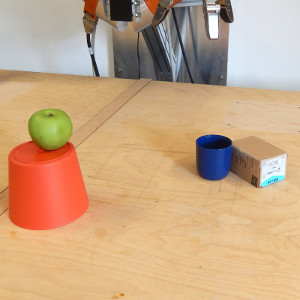
\includegraphics[height=2cm]{./figures/sec/scene_photos/affordance_scene4.jpg}
          & 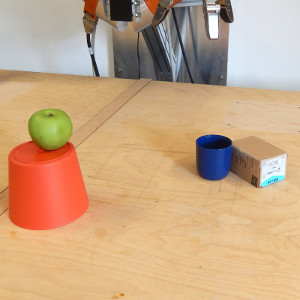
\includegraphics[height=2cm]{./figures/sec/scene_photos/affordance_scene4.jpg}
          & 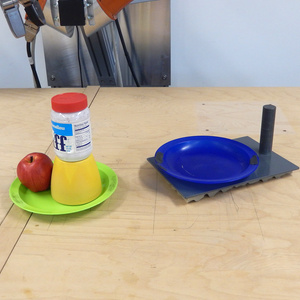
\includegraphics[height=2cm]{./figures/sec/scene_photos/affordance_scene7.jpg}
          & 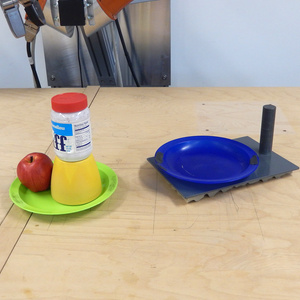
\includegraphics[height=2cm]{./figures/sec/scene_photos/affordance_scene7.jpg}
          & 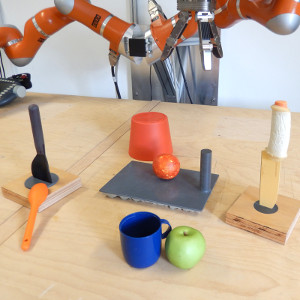
\includegraphics[height=2cm]{./figures/sec/scene_photos/affordance_scene5.jpg}
          & 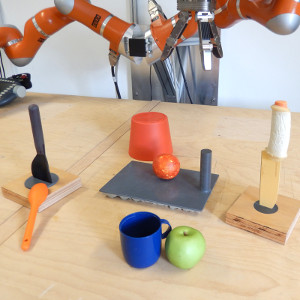
\includegraphics[height=2cm]{./figures/sec/scene_photos/affordance_scene5.jpg}\\
    \multicolumn{2}{l}{Main object}       & Apple           & Cup             & Apple             & Yellow pedestal   & Orange    & Apple\\
    \multicolumn{2}{l}{Primary object}    & Red pedestal    & Box             & Yellow pedestal   & Green plate       & Board     & Cup\\
    \multicolumn{2}{l}{Secondary object}  & Box             & Red pedestal    & Blue plate        & Blue plate        & Cup       & Board\\
    \midrule
    1   & punch         & \checkmark    & \checkmark    & \checkmark    & \checkmark    & \checkmark    & \checkmark\\
    2   & flick         & \checkmark    & \checkmark    & \checkmark    & \checkmark    & \checkmark    & \checkmark\\
    3   & poke          & \checkmark    & \checkmark    & \checkmark    & \checkmark    & \checkmark    & \checkmark\\
    4   & chop          & \checkmark    & \xmark        & \xmark        & \xmark        & \checkmark    & \xmark\\
    5   & bore          & \checkmark    & \checkmark    & \checkmark    & \checkmark    & \checkmark    & \checkmark\\
    6   & cut           & \checkmark    & \xmark        & \xmark        & \xmark        & \checkmark    & \xmark\\
    7   & scratch       & \checkmark    & \checkmark    & \checkmark    & \checkmark    & \checkmark    & \checkmark\\
    8   & scissor-cut   & \checkmark    & \xmark        & \xmark        & \xmark        & \checkmark    & \xmark\\
    9   & squash        & \checkmark    & \checkmark    & \checkmark    & \xmark        & \checkmark    & \checkmark\\
    10  & draw          & \checkmark    & \checkmark    & \checkmark    & \checkmark    & \checkmark    & \checkmark\\
    11  & push          & \checkmark    & \checkmark    & \checkmark    & \xmark        & \checkmark    & \checkmark\\
    12  & stir          & \nmark        & \nmark        & \nmark        & \nmark        & \nmark        & \nmark\\
    13  & knead         & \checkmark    & \checkmark    & \checkmark    & \xmark        & \checkmark    & \checkmark\\
    14  & rub           & \checkmark    & \checkmark    & \checkmark    & \checkmark    & \checkmark    & \checkmark\\
    15  & lever         & \nmark        & \nmark        & \nmark        & \nmark        & \nmark        & \nmark\\
    16  & scoop         & \checkmark    & \checkmark    & \checkmark    & \xmark        & \checkmark    & \checkmark\\
    17  & take down     & \checkmark    & \xmark        & \xmark        & \xmark        & \checkmark    & \xmark\\
    18  & push down     & \checkmark    & \xmark        & \xmark        & \xmark        & \checkmark    & \xmark\\
    19  & rip off       & \checkmark    & \xmark        & \xmark        & \xmark        & \checkmark    & \xmark\\
    20  & break off     & \nmark        & \nmark        & \nmark        & \nmark        & \nmark        & \nmark\\
    \multirow{2}{*}{21} & uncover by    & \multirow{2}{*}{\nmark}       & \multirow{2}{*}{\nmark}       & \multirow{2}{*}{\nmark}   & \multirow{2}{*}{\nmark}    & \multirow{2}{*}{\nmark}    & \multirow{2}{*}{\nmark}\\
      & pick\&place     &               &               &               &               &               &\\
    \multirow{2}{*}{22} & uncover by    & \multirow{2}{*}{\nmark}       & \multirow{2}{*}{\nmark}       &     \multirow{2}{*}{\nmark}   & \multirow{2}{*}{\nmark}    & \multirow{2}{*}{\nmark}    & \multirow{2}{*}{\nmark}\\
      & pushing         &               &               &               &               &               &\\
    23  & put on top    & \checkmark    & \xmark        & \checkmark    & \xmark        & \checkmark    & \xmark\\
    24  & push on top   & \xmark        & \xmark        & \xmark        & \xmark        & \xmark        & \xmark\\
    25  & put over      & \nmark        & \nmark        & \nmark        & \nmark        & \nmark        & \nmark\\
    26  & push over     & \nmark        & \nmark        & \nmark        & \nmark        & \nmark        & \nmark\\
    27  & grasp         & \checkmark    & \checkmark    & \checkmark    & \xmark        & \checkmark    & \checkmark\\
    28  & push apart    & \xmark        & \checkmark    & \checkmark    & \xmark        & \xmark        & \checkmark\\
    29  & push together & \xmark        & \xmark        & \xmark        & \xmark        & \xmark        & \xmark\\
    30  & grasp         & \checkmark    & \checkmark    & \checkmark    & \xmark        & \checkmark    & \checkmark\\
    \bottomrule
    \caption{The different scenes are enlarged in \figref{fig:sec_enriched_geometricalreasoning_experiments_scenesexample}.
    Please note that one cannot check the preconditions for some actions, \eg stirring, knead which are related to the material of objects.
    These actions are denoted with ``\nmark''; they require high level object knowledge.
    A ``\checkmark'' denotes executability of the action; the actions ``\xmark'' were correctly computed as not possible to execute.}
    \label{tab:affordanceofsemanticeventchains_sceneresults}
  \end{longtable}
\end{landscape}
}
\normalsize




\subsection{Using affordance for planning}

In this section the system is evaluated using four different scenarios.
The experimental setup is as follows:

\begin{enumerate}
  \item \textbf{Push object 1 to object 2.} In the first scenario the task is to push the \emph{main} object, a red apple, to the \emph{secondary} object, a yellow pedestal. Another object is touching the \emph{secondary} object.
  \item \textbf{Pick and place from tower structure.} The second scenario contains a tower structure as shown in \figref{fig:sec_structuralinformation_structures_3}. The robot needs to pick and place a cutting board with fruits and needs to empty the board first.
  \item \textbf{Pour liquid.} The robot needs to pour a liquid into a bowl. Currently, the bowl is used for fruits and needs to be emptied first. For the liquid colored sand is used\footnote{Experiments have shown that using real liquids for robot experiments lead to messy problems.}.
  \item \textbf{Cut cucumber.} The robot has to cut a cucumber on top of a board. The board is occupied by an apple and needs to be cleaned first.
\end{enumerate}

Qualitative results for execution are shown in \figref{fig:sec_usingaffordanceforplanning_results_scenario1}, \figref{fig:sec_usingaffordanceforplanning_results_scenario2}, \figref{fig:sec_usingaffordanceforplanning_results_scenario3}, and \figref{fig:sec_usingaffordanceforplanning_results_scenario4}; corresponding to scenarios 1, 2, 3, and 4. 
In the next sections, we will review and discuss the findings.





\subsubsection{Results for scenario 1}

The task given to the robot system is \action{push the red apple to the pedestal}.
The first keyframe of the scene is shown in \figref{fig:sec_usingaffordanceforplanning_results_scenario1_1}, the respective graph relations are as follows

\begin{align*}
  \bordermatrix{
    & \textup{Table}     & \textup{Green apple}   & \textup{Pedestal}  & \textup{Red apple}\cr
    \textup{Table (id = 0)}        & \colorbox{green120}{0} & \textup{T} & \textup{T} & \textup{T}\cr
    \textup{Green apple (id = 1)} & \textup{T} & \colorbox{green120}{1} & \textup{T} & \textup{N}\cr
    \textup{Pedestal (id = 2)}     & \textup{T} & \textup{T} & \colorbox{green120}{2} & \textup{N}\cr
    \textup{Red apple (id = 3)}   & \textup{T} & \textup{N} & \textup{N} & \colorbox{green120}{3}\cr
    }.
\end{align*}

The \emph{main} object is only contained in one subgraph: one single object on top of the support (cf. \figref{fig:sec_structuralinformation_structures_1}), which is, as shown in \tabref{tab:sec_usingaffordanceforplanning_preconditions}, allowed for the action \action{push}.
Also, the preconditions for the \emph{secondary} object are met.
This is the trivial case, where the current scene already affords the preconditions of the target action.
This means, that no further planning is required.
After executing the action, the resulting subgraph will consist of one structure containing two touching objects on top of one support (cf. \figref{fig:sec_structuralinformation_structures_2}).
Keyframes showing the robot performing the requested action are listed in \figref{fig:sec_usingaffordanceforplanning_results_scenario1}. 

\begin{figure}
  \centering
  \begin{subfigure}[t]{0.475\textwidth}
    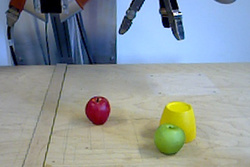
\includegraphics[width=\textwidth]{./figures/sec/planning/exec1/frame0548.jpg}
    \caption{Keyframe 1.}
    \label{fig:sec_usingaffordanceforplanning_results_scenario1_1}
  \end{subfigure}
  \hfill
  \begin{subfigure}[t]{0.475\textwidth}
    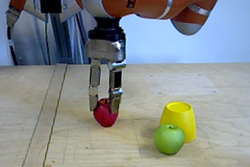
\includegraphics[width=\textwidth]{./figures/sec/planning/exec1/frame0816.jpg}
    \caption{Keyframe 2.}
    \label{fig:sec_usingaffordanceforplanning_results_scenario1_2}
  \end{subfigure}\\%
  \begin{subfigure}[t]{0.475\textwidth}
    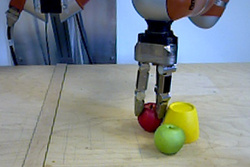
\includegraphics[width=\textwidth]{./figures/sec/planning/exec1/frame0924.jpg}
    \caption{Keyframe 3.}
    \label{fig:sec_usingaffordanceforplanning_results_scenario1_3}
  \end{subfigure}
  \hfill
  \begin{subfigure}[t]{0.475\textwidth}
    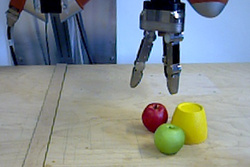
\includegraphics[width=\textwidth]{./figures/sec/planning/exec1/frame1021.jpg}
    \caption{Keyframe 4.}
    \label{fig:sec_usingaffordanceforplanning_results_scenario1_4}
  \end{subfigure}
  \caption{Scenario 1: The red apple is being pushed to the pedestal, which is touched by another apple.}
  \label{fig:sec_usingaffordanceforplanning_results_scenario1}
\end{figure}





\subsubsection{Results for scenario 2}

\Figref{fig:sec_usingaffordanceforplanning_results_scenario2} depicts the second scenario. 
The task given to the planner is to \action{pick and place the cutting board on top of the plate}. 
From the first keyframe the following graph is extracted:

\begin{align*}
  \bordermatrix{
                                    & \textup{Table}        & \textup{R. apple}     & \textup{G. apple}     & \textup{C. board}& \textup{Plate}\cr
    \textup{Table (id = 0)}         & \colorbox{green120}{0}& \textup{N}            & \textup{N}            & \textup{T}            & \textup{T}\cr
    \textup{Red apple (id = 1)}     & \textup{N}            & \colorbox{green120}{1}& \textup{N}            & \textup{T}            & \textup{N}\cr
    \textup{Green apple (id = 2)}   & \textup{N}            & \textup{N}            & \colorbox{green120}{2}& \textup{T}            & \textup{N}\cr
    \textup{Cutting board (id = 3)} & \textup{T}            & \textup{T}            & \textup{T}            & \colorbox{green120}{3}& \textup{N}\cr
    \textup{Plate (id = 4)}         & \textup{T}            & \textup{N}            & \textup{N}            & \textup{N}            & \colorbox{green120}{4}\cr
    }
\end{align*}

where ``R. apple'' is short for ``Red apple'', ``G. apple'' for ``Green apple'', and ``C. board'' stands for ``Cutting board''.
On the semantic level the planner extracts three subgraphs around the \emph{main} object: two are tower structures (cf. \figref{fig:sec_structuralinformation_structures_3}) and not allowed for the pick and place action.
The third one is one single object on top of the support, which is allowed for \action{pick and place}.
First, the planner suggests to remove the red apple via pick and place onto the table.
As the requested action is still not allowed, as one tower structure remains, a second pick and place action of the green apple is added to the list.
Eventually, the cutting board is free of any other objects and can be picked and placed on top of the plate.
The removal sequence of the fruits depends on the object enumeration; in the shown case the red apple is removed first as it has a lower object identifier. 
Successful execution of the plan

\begin{enumerate}
  \item \action{Pick and place red apple on top of table},
  \item \action{Pick and place green apple on top of table}, and
  \item \action{Pick and place cutting board on top of plate}.
\end{enumerate}

is demonstrated in \figref{fig:sec_usingaffordanceforplanning_results_scenario2}.

\begin{figure}
  \centering
  \begin{subfigure}[t]{0.475\textwidth}
    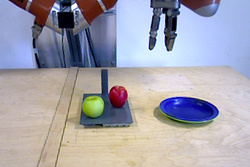
\includegraphics[width=\textwidth]{./figures/sec/planning/exec2/frame0511.jpg}
    \caption{Keyframe 1.}
    \label{fig:sec_usingaffordanceforplanning_results_scenario2_1}
  \end{subfigure}
  \hfill
  \begin{subfigure}[t]{0.475\textwidth}
    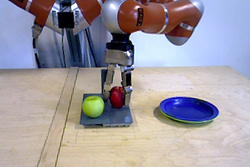
\includegraphics[width=\textwidth]{./figures/sec/planning/exec2/frame0837.jpg}
    \caption{Keyframe 2.}
    \label{fig:sec_usingaffordanceforplanning_results_scenario2_2}
  \end{subfigure}\\%
  \begin{subfigure}[t]{0.475\textwidth}
    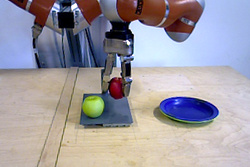
\includegraphics[width=\textwidth]{./figures/sec/planning/exec2/frame0892.jpg}
    \caption{Keyframe 3.}
    \label{fig:sec_usingaffordanceforplanning_results_scenario2_3}
  \end{subfigure}
  \hfill
  \begin{subfigure}[t]{0.475\textwidth}
    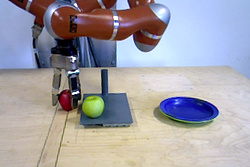
\includegraphics[width=\textwidth]{./figures/sec/planning/exec2/frame1066.jpg}
    \caption{Keyframe 4.}
    \label{fig:sec_usingaffordanceforplanning_results_scenario2_4}
  \end{subfigure}\\%
  \begin{subfigure}[t]{0.475\textwidth}
    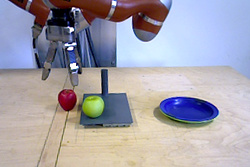
\includegraphics[width=\textwidth]{./figures/sec/planning/exec2/frame1164.jpg}
    \caption{Keyframe 5.}
    \label{fig:sec_usingaffordanceforplanning_results_scenario2_5}
  \end{subfigure}
  \hfill
  \begin{subfigure}[t]{0.475\textwidth}
    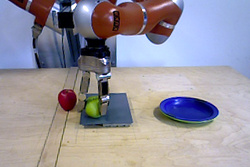
\includegraphics[width=\textwidth]{./figures/sec/planning/exec2/frame2164.jpg}
    \caption{Keyframe 6.}
    \label{fig:sec_usingaffordanceforplanning_results_scenario2_6}
  \end{subfigure}
\end{figure}
\begin{figure}\ContinuedFloat
  \centering
  \begin{subfigure}[t]{0.475\textwidth}
    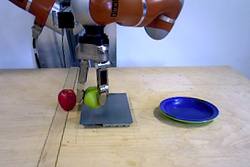
\includegraphics[width=\textwidth]{./figures/sec/planning/exec2/frame2212.jpg}
    \caption{Keyframe 7.}
    \label{fig:sec_usingaffordanceforplanning_results_scenario2_7}
  \end{subfigure}
  \hfill
  \begin{subfigure}[t]{0.475\textwidth}
    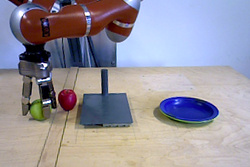
\includegraphics[width=\textwidth]{./figures/sec/planning/exec2/frame2395.jpg}
    \caption{Keyframe 8.}
    \label{fig:sec_usingaffordanceforplanning_results_scenario2_8}
  \end{subfigure}\\%
  \begin{subfigure}[t]{0.475\textwidth}
    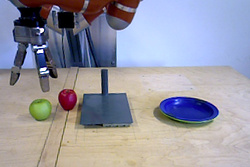
\includegraphics[width=\textwidth]{./figures/sec/planning/exec2/frame2493.jpg}
    \caption{Keyframe 9.}
    \label{fig:sec_usingaffordanceforplanning_results_scenario2_9}
  \end{subfigure}
  \hfill
  \begin{subfigure}[t]{0.475\textwidth}
    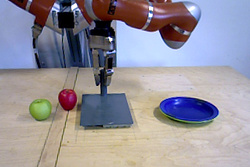
\includegraphics[width=\textwidth]{./figures/sec/planning/exec2/frame3592.jpg}
    \caption{Keyframe 10.}
    \label{fig:sec_usingaffordanceforplanning_results_scenario2_10}
  \end{subfigure}\\%
  \begin{subfigure}[t]{0.475\textwidth}
    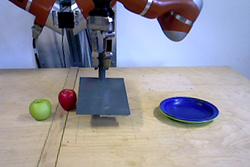
\includegraphics[width=\textwidth]{./figures/sec/planning/exec2/frame3663.jpg}
    \caption{Keyframe 11.}
    \label{fig:sec_usingaffordanceforplanning_results_scenario2_11}
  \end{subfigure}
  \hfill
  \begin{subfigure}[t]{0.475\textwidth}
    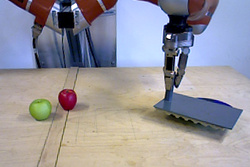
\includegraphics[width=\textwidth]{./figures/sec/planning/exec2/frame3985.jpg}
    \caption{Keyframe 13.}
    \label{fig:sec_usingaffordanceforplanning_results_scenario2_13}
  \end{subfigure}
\end{figure}
\begin{figure}\ContinuedFloat
  \centering
  \begin{subfigure}[t]{0.475\textwidth}
    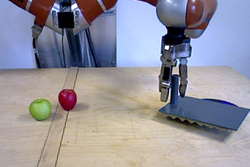
\includegraphics[width=\textwidth]{./figures/sec/planning/exec2/frame4081.jpg}
    \caption{Keyframe 14.}
    \label{fig:sec_usingaffordanceforplanning_results_scenario2_14}
  \end{subfigure}
  \caption{Scenario 2: The robot needs to put a cutting board on top of another plate. For this it needs to empty the board first.}
  \label{fig:sec_usingaffordanceforplanning_results_scenario2}
\end{figure}





\subsubsection{Results for scenario 3}

Scenario 3 holds five objects: a table ($\text{id} = 0$) acts as support, a bowl ($\text{id} = 1$), an apple ($\text{id} = 2$), and a bottle ($\text{id} = 3$).
The fifth object, sauce ($\text{id} = 4$), is at the beginning hidden inside the bottle and not visible to the computer vision system.
The extracted graph structure as created from keyframe \figref{fig:sec_usingaffordanceforplanning_results_scenario3_1} does therefore not contain sauce at the beginning.
It is rather added as soon as it becomes visible and marked ``absent'' (A) in prior graphs of the \gls{ac:sec}:

\begin{align*}
  \bordermatrix{
                                & \textup{Table}        & \textup{Bowl}         & \textup{Red apple}    & \textup{Bottle}       & \textup{Sauce}\cr
    \textup{Table (id = 0)}     & \colorbox{green120}{0}& \textup{T}            & \textup{N}            & \textup{T}            & \textup{A}\cr
    \textup{Bowl (id = 1)}      & \textup{T}            & \colorbox{green120}{1}& \textup{T}            & \textup{N}            & \textup{A}\cr
    \textup{Red apple (id = 2)} & \textup{N}            & \textup{T}            & \colorbox{green120}{2}& \textup{N}            & \textup{A}\cr
    \textup{Bottle (id = 3)}    & \textup{T}            & \textup{N}            & \textup{N}            & \colorbox{green120}{3}& \textup{A}\cr
    \textup{Sauce (id = 4)}     & \textup{A}            & \textup{A}            & \textup{A}            & \textup{A}            & \colorbox{green120}{4}\cr
    }
\end{align*}

Furthermore, the planning system does not contain high level knowledge about the function of objects; meaning awareness that objects may act as \emph{containers}, which hold a liquid.
As the connection between the action \action{pour} and an object acting as \emph{container} for the liquid is not present, the command \action{pour the sauce into the bowl} will always fail due to absence of the sauce (which is not an allowed structure).
While a high level planner, for example a human being, would of course first look into the bottle for sauce to pour, the command given to the planning system is changed accordingly to \action{pour the bottle into the bowl}.
On the planning domain this is now connected to an action, where not the bottle, but rather the content of the bottle is being poured into the bowl.

The results for the third scenario are detailed in \figref{fig:sec_usingaffordanceforplanning_results_scenario3}. 
The task is to \action{pour liquid from bottle into bowl}.
The \emph{primary} object, the bottle, has only one subgraph: One single object on top of support, which is an allowed structure for \action{pick and place}.
The \emph{main} object, however, the bowl is obstructed with an apple.
Thus, the planner detects a tower structure with the bowl as forbidden element.
The planner suggests to remove the top element, the apple, to afford the requested action.
After the apple is removed, the sauce is being poured into the bowl.
The computed plan is as follows:

\begin{enumerate}
  \item \action{Pick and place red apple on top of table},
  \item \action{Pour bottle into bowl}.
\end{enumerate}

\begin{figure}
  \centering
  \begin{subfigure}[t]{0.475\textwidth}
    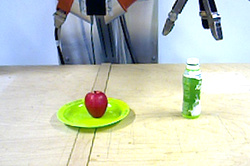
\includegraphics[width=\textwidth]{./figures/sec/planning/exec3/frame0493.jpg}
    \caption{Keyframe 1.}
    \label{fig:sec_usingaffordanceforplanning_results_scenario3_1}
  \end{subfigure}
  \hfill
  \begin{subfigure}[t]{0.475\textwidth}
    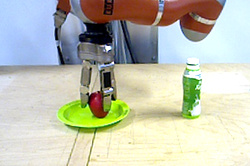
\includegraphics[width=\textwidth]{./figures/sec/planning/exec3/frame0837.jpg}
    \caption{Keyframe 2.}
    \label{fig:sec_usingaffordanceforplanning_results_scenario3_2}
  \end{subfigure}\\%
  \begin{subfigure}[t]{0.475\textwidth}
    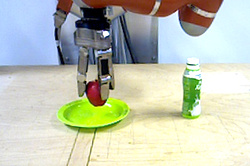
\includegraphics[width=\textwidth]{./figures/sec/planning/exec3/frame0893.jpg}
    \caption{Keyframe 3.}
    \label{fig:sec_usingaffordanceforplanning_results_scenario3_3}
  \end{subfigure}
  \hfill
  \begin{subfigure}[t]{0.475\textwidth}
    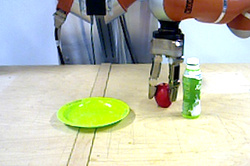
\includegraphics[width=\textwidth]{./figures/sec/planning/exec3/frame1095.jpg}
    \caption{Keyframe 4.}
    \label{fig:sec_usingaffordanceforplanning_results_scenario3_4}
  \end{subfigure}\\%
  \begin{subfigure}[t]{0.475\textwidth}
    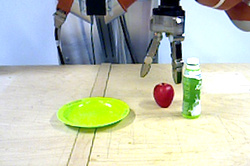
\includegraphics[width=\textwidth]{./figures/sec/planning/exec3/frame1174.jpg}
    \caption{Keyframe 5.}
    \label{fig:sec_usingaffordanceforplanning_results_scenario3_5}
  \end{subfigure}
  \hfill
  \begin{subfigure}[t]{0.475\textwidth}
    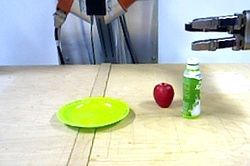
\includegraphics[width=\textwidth]{./figures/sec/planning/exec3/frame2222.jpg}
    \caption{Keyframe 6.}
    \label{fig:sec_usingaffordanceforplanning_results_scenario3_6}
  \end{subfigure}
\end{figure}
\begin{figure}\ContinuedFloat
  \centering
  \begin{subfigure}[t]{0.475\textwidth}
    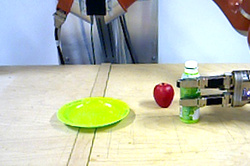
\includegraphics[width=\textwidth]{./figures/sec/planning/exec3/frame2366.jpg}
    \caption{Keyframe 7.}
    \label{fig:sec_usingaffordanceforplanning_results_scenario3_7}
  \end{subfigure}
  \hfill
  \begin{subfigure}[t]{0.475\textwidth}
    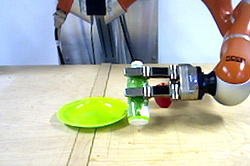
\includegraphics[width=\textwidth]{./figures/sec/planning/exec3/frame2561.jpg}
    \caption{Keyframe 8.}
    \label{fig:sec_usingaffordanceforplanning_results_scenario3_8}
  \end{subfigure}\\%
  \begin{subfigure}[t]{0.475\textwidth}
    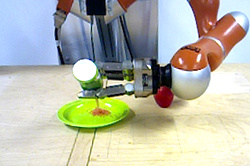
\includegraphics[width=\textwidth]{./figures/sec/planning/exec3/frame2799.jpg}
    \caption{Keyframe 9.}
    \label{fig:sec_usingaffordanceforplanning_results_scenario3_9}
  \end{subfigure}
  \hfill
  \begin{subfigure}[t]{0.475\textwidth}
    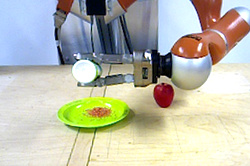
\includegraphics[width=\textwidth]{./figures/sec/planning/exec3/frame2912.jpg}
    \caption{Keyframe 10.}
    \label{fig:sec_usingaffordanceforplanning_results_scenario3_10}
  \end{subfigure}\\%
  \begin{subfigure}[t]{0.475\textwidth}
    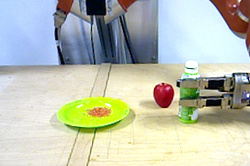
\includegraphics[width=\textwidth]{./figures/sec/planning/exec3/frame3219.jpg}
    \caption{Keyframe 11.}
    \label{fig:sec_usingaffordanceforplanning_results_scenario3_11}
  \end{subfigure}
  \hfill
  \begin{subfigure}[t]{0.475\textwidth}
    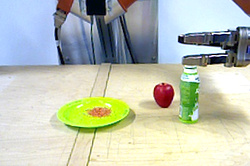
\includegraphics[width=\textwidth]{./figures/sec/planning/exec3/frame3253.jpg}
    \caption{Keyframe 12.}
    \label{fig:sec_usingaffordanceforplanning_results_scenario3_12}
  \end{subfigure}
  \caption{Scenario 3: The robot needs to \action{pour liquid into a bowl}. Currently, the bowl is used for fruits and needs to be cleaned first.}
  \label{fig:sec_usingaffordanceforplanning_results_scenario3}
\end{figure}





\subsubsection{Results for scenario 4}
\label{sssec:action_results_usingaffordanceforplanning_resultsforscenario4}

The fourth scenario can be seen in \figref{fig:sec_usingaffordanceforplanning_results_scenario4}. 
The task is to \action{cut the cucumber with the knife}. 
The extracted graph relations are as follows:

\begin{align*}
  \bordermatrix{
                      & \textup{Table}        & \textup{Cucumber}     & \textup{G. apple}     & \textup{C. board}     & \textup{Holder}       & \textup{Knive}\cr
    \textup{Table}    & \colorbox{green120}{0}& \textup{T}            & \textup{N}            & \textup{T}            & \textup{T}            & \textup{N}\cr
    \textup{Cucumber} & \textup{T}            & \colorbox{green120}{1}& \textup{N}            & \textup{N}            & \textup{N}            & \textup{N}\cr
    \textup{G. apple} & \textup{N}            & \textup{N}            & \colorbox{green120}{2}& \textup{T}            & \textup{N}            & \textup{N}\cr
    \textup{C. board} & \textup{T}            & \textup{N}            & \textup{T}            & \colorbox{green120}{3}& \textup{N}            & \textup{N}\cr
    \textup{Holder}   & \textup{T}            & \textup{N}            & \textup{N}            & \textup{N}            & \colorbox{green120}{4}& \textup{T}\cr
    \textup{Knive}    & \textup{N}            & \textup{N}            & \textup{N}            & \textup{N}            & \textup{T}            & \colorbox{green120}{5}\cr
  }
\end{align*}

\begin{figure}[]
  \centering
  % Define block styles
\tikzstyle{block} = [rectangle, fill=white, text centered, minimum height=0.5em, rounded corners=false]
\tikzstyle{arrow} = [draw, -latex]

\usetikzlibrary{decorations.pathreplacing}

\definecolor{red1}{RGB}{160,0,0}
\definecolor{green1}{RGB}{0,160,0}
\definecolor{blue1}{RGB}{0,0,160}

	      
\begin{tikzpicture}[node distance=2cm, auto]
	% Example
	\node [block] (S01) {Table};
	\node [block, above of=S01] (M01) {\textcolor{red1}{Cucumber}};
	\node [block, left of=M01, node distance=4cm]  (O01) {Cutting board};
	\node [block, right of=M01, node distance=4cm] (O02) {Knife holder};
	\node [block, above of=O01] (O03) {Apple};
	\node [block, above of=O02] (O04) {Knife};

	\draw [] (S01.north) to (M01.south);
	\draw [] (S01.north west) to (O01.south);
	\draw [] (S01.north east) to (O02.south);
	\draw [] (O01.north) to (O03.south);
	\draw [] (O02.north) to (O04.south);
\end{tikzpicture}

  \caption{Graph relation of the first keyframe as shown in \figref{fig:sec_usingaffordanceforplanning_results_scenario4_1}. The \emph{main} object ``Cucumber'' is marked in red.}
  \label{fig:sec_usingaffordanceforplanning_results_scenario4_graph1}
\end{figure}

with the graph relations as shown in \figref{fig:sec_usingaffordanceforplanning_results_scenario4_graph1}.
Executing the action \action{cut the cucumber with the knife} results in immediate success.
Both objects, cucumber and knife, are the only objects on top of a support.
High level knowledge, \ie ``a cutting board is needed for that'' is not included on this low level. 
Here, the human has to interfere and include the action \action{pick and place the cucumber on the cutting board} before \action{cutting}.
This results in

\begin{enumerate}
  \item \action{Pick and place the apple on top of the table},
  \item \action{Pick and place the cucumber on top of the cutting board}, and
  \item \action{Cut the cucumber with the knife}.
\end{enumerate}

But it turns out that there is another, more practical problem.
As shown in \figref{fig:sec_usingaffordanceforplanning_results_scenario4} the robot executes the above actions seemingly without any problems.
The preconditions determined for \action{cutting} request that after cutting the \emph{main} object must have a second object right next to it, touching it.
This should be the new object coming into existence and which was cut from the cucumber.
Even for human beings it is hard to say whether the last two keyframes, \figref{fig:sec_usingaffordanceforplanning_results_scenario4_15} and \figref{fig:sec_usingaffordanceforplanning_results_scenario4_16}, contain one or two pieces of cucumber.
The computer vision algorithms fails, too.
An error is propagated to the planning algorithm and subsequently the plan is recomputed as:

\begin{enumerate}
  \item \action{Cut the cucumber with the knife}.
\end{enumerate}

While moving the knife into cutting position, it fell out of the robot's hand and the robot was not able to grasp it again.
Thus, the experiment was aborted by the user.

\begin{figure}
  \centering
  \begin{subfigure}[t]{0.475\textwidth}
    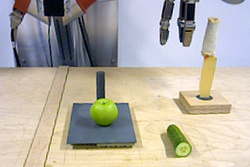
\includegraphics[width=\textwidth]{./figures/sec/planning/exec4/frame0390.jpg}
    \caption{Keyframe 1.}
    \label{fig:sec_usingaffordanceforplanning_results_scenario4_1}
  \end{subfigure}
  \hfill
  \begin{subfigure}[t]{0.475\textwidth}
    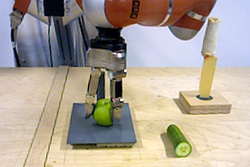
\includegraphics[width=\textwidth]{./figures/sec/planning/exec4/frame0822.jpg}
    \caption{Keyframe 2.}
    \label{fig:sec_usingaffordanceforplanning_results_scenario4_2}
  \end{subfigure}\\%
  \begin{subfigure}[t]{0.475\textwidth}
    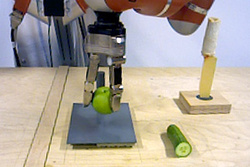
\includegraphics[width=\textwidth]{./figures/sec/planning/exec4/frame0901.jpg}
    \caption{Keyframe 3.}
    \label{fig:sec_usingaffordanceforplanning_results_scenario4_3}
  \end{subfigure}
  \hfill
  \begin{subfigure}[t]{0.475\textwidth}
    \includegraphics[width=\textwidth]{./figures/sec/planning/exec4/frame1068.jpg}
    \caption{Keyframe 4.}
    \label{fig:sec_usingaffordanceforplanning_results_scenario4_4}
  \end{subfigure}\\%
  \begin{subfigure}[t]{0.475\textwidth}
    \includegraphics[width=\textwidth]{./figures/sec/planning/exec4/frame1321.jpg}
    \caption{Keyframe 5.}
    \label{fig:sec_usingaffordanceforplanning_results_scenario4_5}
  \end{subfigure}
  \hfill
  \begin{subfigure}[t]{0.475\textwidth}
    \includegraphics[width=\textwidth]{./figures/sec/planning/exec4/frame2456.jpg}
    \caption{Keyframe 6.}
    \label{fig:sec_usingaffordanceforplanning_results_scenario4_6}
  \end{subfigure}
\end{figure}
\begin{figure}\ContinuedFloat
  \centering
  \begin{subfigure}[t]{0.475\textwidth}
    \includegraphics[width=\textwidth]{./figures/sec/planning/exec4/frame2502.jpg}
    \caption{Keyframe 7.}
    \label{fig:sec_usingaffordanceforplanning_results_scenario4_7}
  \end{subfigure}
  \hfill
  \begin{subfigure}[t]{0.475\textwidth}
    \includegraphics[width=\textwidth]{./figures/sec/planning/exec4/frame2872.jpg}
    \caption{Keyframe 8.}
    \label{fig:sec_usingaffordanceforplanning_results_scenario4_8}
  \end{subfigure}\\%
  \begin{subfigure}[t]{0.475\textwidth}
    \includegraphics[width=\textwidth]{./figures/sec/planning/exec4/frame2951.jpg}
    \caption{Keyframe 9.}
    \label{fig:sec_usingaffordanceforplanning_results_scenario4_9}
  \end{subfigure}
  \hfill
  \begin{subfigure}[t]{0.475\textwidth}
    \includegraphics[width=\textwidth]{./figures/sec/planning/exec4/frame3888.jpg}
    \caption{Keyframe 10.}
    \label{fig:sec_usingaffordanceforplanning_results_scenario4_10}
  \end{subfigure}\\%
  \begin{subfigure}[t]{0.475\textwidth}
    \includegraphics[width=\textwidth]{./figures/sec/planning/exec4/frame4024.jpg}
    \caption{Keyframe 11.}
    \label{fig:sec_usingaffordanceforplanning_results_scenario4_11}
  \end{subfigure}
  \hfill
  \begin{subfigure}[t]{0.475\textwidth}
    \includegraphics[width=\textwidth]{./figures/sec/planning/exec4/frame4450.jpg}
    \caption{Keyframe 12.}
    \label{fig:sec_usingaffordanceforplanning_results_scenario4_12}
  \end{subfigure}
\end{figure}
\begin{figure}\ContinuedFloat
  \centering
  \begin{subfigure}[t]{0.475\textwidth}
    \includegraphics[width=\textwidth]{./figures/sec/planning/exec4/frame5746.jpg}
    \caption{Keyframe 13.}
    \label{fig:sec_usingaffordanceforplanning_results_scenario4_13}
  \end{subfigure}
  \hfill
  \begin{subfigure}[t]{0.475\textwidth}
    \includegraphics[width=\textwidth]{./figures/sec/planning/exec4/frame4450.jpg}
    \caption{Keyframe 14.}
    \label{fig:sec_usingaffordanceforplanning_results_scenario4_14}
  \end{subfigure}\\%
  \begin{subfigure}[t]{0.475\textwidth}
    \includegraphics[width=\textwidth]{./figures/sec/planning/exec4/frame5803.jpg}
    \caption{Keyframe 15.}
    \label{fig:sec_usingaffordanceforplanning_results_scenario4_15}
  \end{subfigure}
  \hfill
  \begin{subfigure}[t]{0.475\textwidth}
    \includegraphics[width=\textwidth]{./figures/sec/planning/exec4/frame6101.jpg}
    \caption{Keyframe 16.}
    \label{fig:sec_usingaffordanceforplanning_results_scenario4_16}
  \end{subfigure}\\%
  \begin{subfigure}[t]{0.475\textwidth}
    \includegraphics[width=\textwidth]{./figures/sec/planning/exec4/frame6211.jpg}
    \caption{Keyframe 17.}
    \label{fig:sec_usingaffordanceforplanning_results_scenario4_17}
  \end{subfigure}
  \caption{Scenario 4: The robot needs to cut a cucumber. At the beginning the cutting board is occupied by an apple, which must be removed first.}
  \label{fig:sec_usingaffordanceforplanning_results_scenario4}
\end{figure}

This outlines numerous problems.
First, the action \action{cut the cucumber with the knife} was executed incorrectly; meaning the cucumber was to be cut on the table instead of the cutting board.
It becomes clear that some actions require high level knowledge for correct execution.
From the list in \tabref{tab:sec_definitionofactions_actiontable} this includes \action{chop}, \action{cut}, \action{draw}, \action{stir}, \action{lever}, and \action{scoop}:

\begin{itemize}
  \item \action{Chop}: Chopping should be performed on top of a stable support. This is the same problem which is mentioned above.
  \item \action{Cut}: See \action{Chop}.
  \item \action{Draw}: One can argue about \action{drawing} that it needs a certain amount of creativity or at least information on about what to draw. However, trajectory planning is also required for all other actions. While these trajectories usually can be generated from low level information (\eg move the arm from point A to B and avoid obstacles while doing this), drawing needs more detailed instructions. The same could be said about \action{poke}, \action{knead}, or \action{rub}.
  \item \action{Stir}: The \gls{ac:sec} domain contains no information about object details, for example as viscosity. Consequently, there is no information whether an object might be stirred.
  \item \action{Lever}: The intent of \action{levering} is moving a heavy object. Again, however, no detailed object information is available (as ``Is this object too heavy to lift?''). Moreover, levering needs very precise information on how to use the lever: this information is not always available to the robot.
  \item \action{Scoop}: See \action{Stir}.
\end{itemize}

In conclusion of the first error one could add a symbolic planner on top of the \gls{ac:sec} planner.
This is discussed in the next session.

Second, there is the sensor problem that the cucumber was not detected as being successfully cut.
The here utilized experiment setup is vision based.
One could add other sensors provided by the robot: for example force or the mere fact that the knife has cut through the cucumber and touched the board.
Especially the second fact can often be detected on the relation graphs and the generation of keyframe \figref{fig:sec_usingaffordanceforplanning_results_scenario4_13} shows that it indeed was detected here.
When to trust vision and when to trust relation graphs (which also are generated from vision here!) is another question.
As neither has a score measuring uncertainty, this remains an open question.

Lastly, there is the hardware problem that the robot drops the knife.
The cutting movement rocked the knife such that the robot's grip became unstable.
Even though the robot's hand contains force feedback sensors, this was not detected.
After the knife fell down, the robot is not able to grasp it again in a secure manner or rotate the knife such that the sharp edge points downwards.
However, what one could do in such an event is to define an error routine:

\begin{enumerate}
  \item \action{Pick and place the knife into the knife holder},
  \item \action{Cut the cucumber with the knife},
\end{enumerate}

where the knife is first put in a well defined position where it can be grabbed again in secure manner.
This error routine is hardware- and action-dependent and does not generalize very well.
Again, it holds higher level knowledge about specific outcomes of specific events.
